% !TEX root =  master.tex
%\section{Zieldefinition}
%Das Ziel dieser Arbeit ist es zum einen die Vorteile von Continuous Integration und Continuous Deployment aufzuzeigen und zum anderen verschiedenen Systeme für CI \& CD untereinander zu vergleichen. Das Aufzeigen der Vorteile wird dabei als Aufhänger genutzt um in das Thema einzuleiten. Der Praxisbezug wird durch das Problem der Abteilung hergestellt. Deren CI/CD Pipeline braucht mittlerweile mehr als 20 Minuten um einen Durchlauf abzuschließen. Aus diesem Grund haben Sie sich dazu entschlossen die Pipeline auf einen Cluster aufzuteilen, dabei übernehmen die einzelnen Knoten im Cluster spezialisierte Aufgaben. Ein Knoten kümmert sich zum Beispiel um die Unit-Tests und ein weiterer um Komponententests durchzuführen. Dadurch soll die Zeit für eine Durchlauf reduziert werden. Um diese Cluster aufzubauen gibt es viele Möglichkeiten von vielen Anbietern. Sowohl in der Cloud als auch On Premise. Da die Ressourcen der Abteilung beschränkt sind wollen sie natürlich die am Besten zu ihnen passende Lösung. Mit dieser Problemstellung wird sich diese Arbeit größtenteils beschäftigen. Am Ende der Arbeit soll eine Handlungsempfehlung für die Abteilung vorliegen an der sie sich orientieren kann.
%\section{Untersuchungsmethodik}
%Damit die Alternativen möglichst objektiv bewertet werden können soll eine AHP-Analyse(Analytic Hierarchy Process) durchgeführt werden. Dabei ist das Ziel möglichst viele Stakeholder an der Aufstellung des Kriterienkatalogs und der Gewichtung teilhaben zu lassen.
\chapter{Einleitung}
\begin{center}\textbf{\enquote{Das muss man doch auch automatisieren können!?}}\end{center}
So oder so ähnlich muss es jedem Entwickler oder auch Administrator schon einmal durch den Kopf gegangen sein. Sei es bei einfachen repetitiven Aufgaben wie zum Beispiel das Anlegen eines neuen Users, oder auch beim Administrieren von großen Serverclustern. Und damit haben sie auch Recht. Mittlerweile gibt es unzählige Tools, die genau solche Aufgaben auf einfache Art und Weise automatisieren können.\\
Doch warum dort mit der Automatisierung stoppen?\\
Schon während der Entwicklung lassen sich viele Schritte automatisieren. Dies steigert die Geschwindigkeit des Entwicklungsprozesses und schont die Nerven der Entwickler.
\section{Motivation}
Möglich gemacht wird dies durch sogenannte Continuous Practices (\ac{CI}, \ac{CDE} und \ac{CD}) (siehe \ref{CP}). Sie helfen dem Entwickler(-team) dabei, ihre Entwicklungen zu \enquote{bauen}, zu testen und falls es entsprechend konfiguriert ist, auch zu veröffentlichen beziehungsweise auf entsprechenden Systemen zu installieren.\\ Dies steigert die Flexibilität und Agilität der Entwickler und verkürzt die Time-to-Market (also die Zeit, die gebraucht wird, um von der Entwicklung zum fertigen und releasefähigem Produkt zu kommen). Sie können sich viel besser auf die tatsächliche Entwicklung konzentrieren anstatt auf das, was darum herum passiert.\\ Trotz dieser Vorteile sind Continuous Practices nicht so weit verbreitet, wie man denken würde. Laut einer Umfrage (\cite{JetBrains.2016}) benutzten erst 44\% der Entwickler weltweit diese Practices tatsächlich während der Entwicklung.\autocite{JetBrains.2016}  Damit bleibt eine Menge Potential ungenutzt. Viele Unternehmen geben an, dass ihnen geschulte Mitarbeiter für diese Technologien fehlen, außerdem fehlt ihnen schlichtweg die Zeit, um die Prozesse zu automatisieren.\autocite{Claranet.2016}\\ Aus diesem Grund möchte die Abteilung AITs-B\&PS-GER-TEC-AM CAP DB APP NordWest ein Angebot für \ac{CI}/\ac{CDE}/\ac{CD} as a Service erstellen. \enquote{as a Service} bedeutet dabei, dass der Kunde kein eigenes dediziertes System mehr erhält. Stattdessen bezahlt er für die Bereitstellung eines Services in der Cloud. Er bezahlt dabei nur für die Nutzung und nicht das gesamte System. Des Weiteren sind solche Systeme sehr gut skalierbar. Das bedeutet, dass der Kunde bei erhöhtem Leistungsbedarf diese Mehrleistung sehr schnell erhalten kann, ohne dass große Umstellungen getätigt werden müssen.\\ Die Abteilung möchte dem Kunden (intern sowie extern) damit ein möglichst komplettes \ac{CI}/\ac{CDE}/\ac{CD} System bieten, auf dem der Kunde so wenig wie möglich anpassen muss. Vom Hosting bis zu etwaigen Integration von Projekten soll alles angeboten und übernommen werden. 
\section{Problemstellung} 
Wie fängt man bei der Erstellung eines Angebots für \ac{CI}/\ac{CDE}/\ac{CD} as a Service an? Damit man überhaupt etwas anbieten kann, braucht man zunächst einen Service. Doch wie zieht man diesen Service auf? Man kann das komplette System mitsamt \ac{CI}/\ac{CDE}/\ac{CD}-Tools von Grund auf aufbauen. Allerdings würde man sich damit nur extra Arbeit schaffen. Mittlerweile gibt es unzählige Tools für \ac{CI}, \ac{CDE} und \ac{CD}. Viele davon sind spezialisiert auf besondere Anwendungsgebiete, aber es gibt auch einige Allrounder.\\ Doch welches Tool ist jetzt das am besten geeignete für die Anwendung in dem Service? Und wie wähle ich das am besten geeignete Tool aus?\\
Mit diesen Problemstellungen wird sich diese Arbeit im Folgenden beschäftigen. Es wird ein Analyseverfahren ermittelt mithilfe dessen dann verschiedene Alternativen evaluiert werden.
\section{Zielsetzung} 
Ziel dieser Bachelorarbeit ist es, verschiedene \ac{CI}/\ac{CDE}/\ac{CD}-Tools zu evaluieren, um am Ende der Abteilung ein Tool präsentiert zu können, welches mit den Anforderungen der Abteilung am besten übereinstimmt. Die Anforderungen der Abteilung werden vorher erarbeitet und mithilfe eines geeigneten Analyseverfahrens entsprechend ihrer Prioritäten aufgenommen. Dabei werden möglichst viele Stackeholder in den Prozess mit einbezogen, um am Ende ein möglichst objektives Ergebnis zu erhalten.\\
\\
Der Fokus der Arbeit liegt dabei auf dem analytischen Vergleich der verschiedenen Alternativen, welche zuvor eine Vorauswahl durchlaufen, da der Vergleich aller Tools den Rahmen dieser Arbeit sprengen würde. Die Implementierung des \ac{CI}/\ac{CDE}/\ac{CD} as a Service ist kein Teil dieser Arbeit. Des Weiteren  soll mit der Arbeit ein Einblick in das \ac{CI}, \ac{CDE} und \ac{CD} \enquote{Ökosystem} gegeben werden, um damit einen Erkenntnisgewinn für die Abteilung zu erhalten.
\chapter{Theoretische Grundlagen} 
Im folgenden Abschnitt werden die theoretischen Grundlagen geschaffen, die für das Verständnis dieser Arbeit relevant sind. Auf der technischen Seite werden sowohl Continuous Integration und Continuous Deployment als auch Versionsverwaltungssysteme erläutert. Ein Überblick über die Methodik der Arbeit wird mit der AHP-Analyse gegeben.
\section{Analytic Hierarchy Process (AHP-Analyse)}\label{ahp}
Wie kann man rationale Entscheidungen in einer irrationalen Welt treffen? Man kann es nicht. Allerdings ist es möglich, mithilfe von verschiedenen Analysemethoden der Entscheidungstheorie eine möglichst große Näherung an eine rationale Entscheidung zu erreichen. 
\subsection{Einführung}
Eine dieser Methoden ist die \ac{NWA}. Sie ist ein bewährtes Hilfsmittel in Wissenschaft und Wirtschaft, um Entscheidungen zu finden und Möglichkeiten zu bewerten. Indem das Problem fragmentiert wird, kann durch die Methodik der Nutzwertanalyse die vollständige Problematik erfasst werden, oder anders ausgedrückt: \enquote{Das Gesamtproblem, das es zu entscheiden gilt, wird in Teilprobleme zerlegt und diese, wenn erforderlich, wiederum in Teilprobleme}\autocite[S.1]{Kuehnapfel.2014}. Alle Facetten des Problems werden betrachtet und nicht vereinfacht oder abstrahiert. Somit umgeht man die menschliche Natur, die aufgrund einer möglichen Zeitersparnis ein komplexes Problem immer vereinfachen will. Das Vereinfachen führt allerdings zu einer erhöhten Fehlerquote und zum sofortigen Ausschluss von unkonventionellen Möglichkeiten aufgrund der Tendenz des Menschen zu Konstanz und Bewahrung\autocite[Vgl.][S.1]{Kuehnapfel.2014}. Im Gegensatz dazu gewährleistet die Nutzwertanalyse Objektivität und Chancengleichheit unter den verschiedenen Alternativen.\newline
Die Rationalität der Methodik ergibt sich aus der Vorgehensweise bei der Bearbeitung einer Fragestellung. Die einzelnen Fragmente (Kriterien) der Fragestellung werden einzeln bewertet und entsprechend ihrer Relevanz für das Gesamtproblem gewichtet.\autocite[Vgl.][S.10]{Kuehnapfel.2014} An der Auswahl der Kriterien und deren Gewichtung sollten möglichst viele Stackeholder beteiligt sein, um die Einflussnahme einzelner Meinungen zu unterbinden.\\
\\
In den 1970er Jahren hat Thomas L. Saaty das Konzept der \ac{NWA} weiterentwickelt. Der \ac{AHP} ist wie die \ac{NWA} ein grundlegender Ansatz zur Entscheidungsfindung und wurde entworfen, um sowohl rationale als auch intuitive Entscheidungen in die Auswahl von zuvor selektierten Alternativen einzubeziehen.\autocite[Vgl.][S.1]{Saaty.2012} Er heißt Analytischer Hierarchie Prozess, weil er sowohl analytisch, hierarchisch als auch prozessorientiert arbeitet.\autocite{TUM.2015}
\begin{itemize}
	\item\texttt{analytisch:} Die Entscheidungsunterstützung erfolgt mathematisch und mittels Logik
	\item\texttt{hierarchisch:} \enquote{Bei Nutzung des AHP sind die für die Erfüllung der Zielstellung genutzten Entscheidungskriterien einer hierarchischen Struktur unterworfen.}\autocite[S.314]{Hausladen.2016} 
	\item\texttt{prozessorientiert:} Die Entscheidungsunterstützung erfolgt immer nach demselben Prozess
\end{itemize}
Während des Prozesses werden einfache paarweise Vergleiche durchgeführt. Die Ergebnisse dieser Vergleiche werden dann genutzt, um eine Reihenfolge der Alternativen zu erstellen.\autocite[Vgl.][S.1]{Saaty.2012}
\subsection{Ablauf des AHP}
Die einfachste Form, ein Entscheidungsproblem in einer AHP-Analyse darzustellen, ist die innerhalb einer Hierarchie mit drei Ebenen.(Abbildung \ref{img:hier})
\begin{figure}[h!]
	\centering
	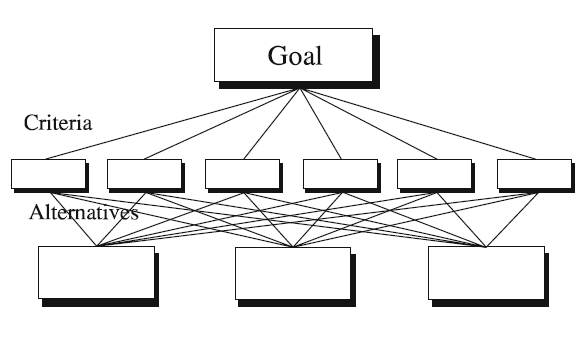
\includegraphics[scale = 0.8]{img/Hierarchie.png}
	\quelle{\cite[S.3]{Saaty.2012}}
	\caption{three level hierarchie}
	\label{img:hier}
\end{figure}
Das Grundproblem wird immer weiter granuliert. Auf der untersten Ebene finden sich die Alternativen, welche mithilfe der Kriterien auf Ebene 2 evaluiert werden. Diese Erkenntnisse werden dann genutzt, um das Ziel der Entscheidung auf der obersten Ebene zu bestimmen.\autocite[Vgl.][S.2]{Saaty.2012}
Damit hat man auch gleich den Startpunkt einer AHP-Analyse bestimmt. 
\subsubsection{Aufstellen des Entscheidungsmodells}
Die Analyse beginnt wie oben bereits beschrieben mit dem Aufstellen des hierarchischen Entscheidungsmodells. Aus dem Entscheidungsproblem wird ein Ziel definiert, welchem eine endliche Anzahl von Alternativen zugeordnet wird $X=\{x_{1}, ..., x_{n}\}$\autocite[Vgl.][S.3]{Brunelli.2015}.
Des Weiteren werden die Kriterien auf deren Basis die Alternativen verglichen werden aus dem Ziel abgeleitet. Sollte die Kriterienanzahl zu groß sein bietet es sich an, diese in Subkriterien aufzuteilen. Dadurch erhält man eine weitere Ebene innerhalb der Hierarchie. Am Ende dieser Phase der AHP-Analyse sollte eine Struktur ähnlich zu Abbildung \ref{img:hier} vorhanden sein. Mit dieser fertig erstellten Hierarchie erhält man eine bessere Übersicht über die Entscheidung, die gefällt wird, die Kriterien, die genutzt werden und die Alternativen, die zur Verfügung stehen.\autocite[Vgl.][S.9]{Mu.2018} 
\subsubsection{Gewichtung der Kriterien}
Nicht alle Kriterien werden die gleiche Relevanz haben. Deswegen werden im zweiten Schritt der AHP-Analyse die Kriterien gewichtet.\autocite[Vgl.][S.9]{Mu.2018} Diese Gewichtung erfolgt relativ zueinander. Relativ bezieht sich dabei auf den Umstand, dass für die Priorisierung der einzelnen Kriterien diese im Verhältnis zueinander bestimmt werden. \\
Damit die Gewichtungen vergleichbar sind, besonders, wenn diese in einem Bewertungsgremium getroffen werden, muss es eine zentrale Skala geben. Mithilfe dieser werden dann die entsprechenden Gewichtungen vorgenommen. Am Ende diese Prozesses soll ein Gewichtungsvektor $w=(w_{1}, ..., w_{n})$ mit einem $w_i$ für jedes $x_i$ aus $X=\{x_{1}, ..., x_{n}\}$ entstehen\autocite[Vgl.][S.4]{Brunelli.2015}. \\
\begin{figure}[h!]
	\centering
	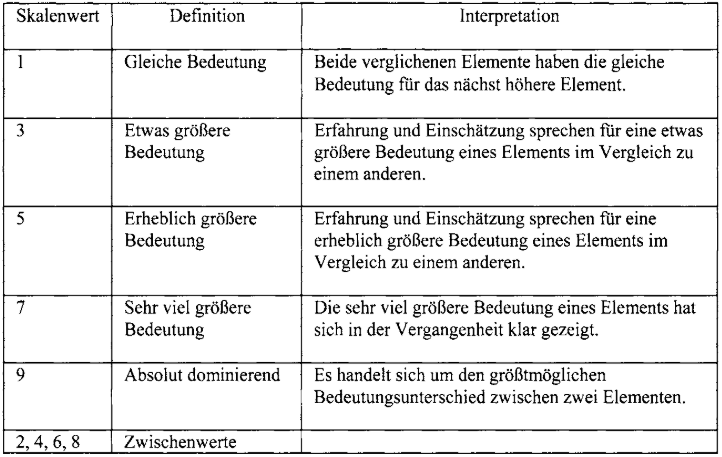
\includegraphics[scale = 0.8]{img/Skala.png}
	\quelle{\cite[S.105]{Fink.2006}}
	\caption{Saaty-Skala}
	\label{img:scale}
\end{figure}
Die Schwierigkeit dabei ist die Auswahl der richtigen/passenden Skala. In seinem 1977 veröffentlichen Artikel\autocite{Saaty.1977} vergleicht Saaty verschiedene Skalen miteinander und kommt dabei zu dem Schluss, dass die Skala von 1-9 (Abbildung \ref{img:scale}) die passendste im Hinblick auf die Anwendung mit der AHP-Analyse ist. \\
Mithilfe dieser Skala werden nun die paarweise Vergleiche durchgeführt. Jede Kategorie wird mit jeder anderen einzeln verglichen und mithilfe der Skala bewertet.\autocite[Vgl.][S.106]{Fink.2006}  
\[\begin{array}{rcl}
		\centering
	  x_1 &\leftrightarrow &x_2 \\
	  x_1 &\leftrightarrow &x_3 \\
	  x_2 &\leftrightarrow &x_3 \\
   \vdots &                &\vdots
\end{array}\]
Am Ende dieses Prozesses sollte eine Matrix ähnlich zu \ref{matrix} entstanden sein.
\begin{table}[h!]
    \centering
\[X\quad = \quad\begin{tabular}{l|llll}
		& $x_1$ & $x_2$ &  $x_3$  \\ \hline
  $x_1$ &   1   &   5   &   2   \\
  $x_2$	&$\frac{1}{5}$&   1   &$\frac{1}{3}$     \\
  $x_3$	&$\frac{1}{2}$&   3   &   1         
   	  \end{tabular} 	  
\quad bzw. \quad
\left( \begin{array}{rrrr}
 1   &   5   &   2   \\
\frac{1}{5}&   1   &\frac{1}{3}     \\
\frac{1}{2}&   3   &   1        
\end{array}\right) 
\]
\caption{Matrix}
\label{matrix}
\end{table}
In diesem Beispiel lässt sich erkennen, dass $x_1$ erheblich größere Bedeutung hat als $x_2$. Außerdem hat $x_3$ etwas größere Bedeutung als $x_2$.
\subsubsection{Gewichtungsvektoren}
Mit dieser Tabelle lassen sich jetzt aber noch keine Aussagen treffen. Deswegen werden in diesem Arbeitsschritt die Gewichtungsvektoren $w=(w_{1}, ..., w_{n})$ berechnet.\\
Hierfür gibt es zwei Methoden: das Näherungsverfahren und die Eigenvektormethode. Die Eigenvektormethode kann dabei als theoretischer Grundbaustein der AHP-Analyse angesehen werden.\autocite[Vgl.][S.106]{Fink.2006} Für die nachfolgende Erklärung wird allerdings das Näherungsverfahren beschrieben. Dieses führt\enquote{im Falle vollkommen konsistenter Urteile ebenfalls zu exakten Ergebnissen}\autocite[S.106]{Fink.2006}.
\begin{figure}[h!]
	\centering
	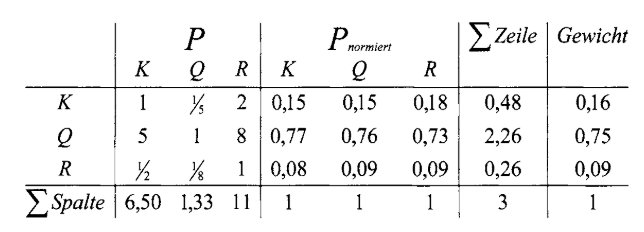
\includegraphics[scale = 0.9]{img/Tabelle.png}
	\quelle{\cite[S.107]{Fink.2006}}
	\caption{Paarvergleichsmatrix}
	\label{img:table}
\end{figure}
Die Berechnung beginnt mit der Normalisierung der Matrix aus dem vorangegangenen Arbeitsschritt. Dafür werden die Spalten zuerst aufsummiert. Danach teilt man jede einzelne Zelle durch die Summe ihrer Spalte. Sobald dies erledigt ist, erhält man das $P_{normiert}$ aus Abbildung \ref{img:table}. Für die abschließenden Gewichtungen müssen jetzt nur noch die Summen der Spalten gebildet werden und durch die Anzahl der Kriterien $n$ geteilt werden. In dem Beispiel \ref{img:table} ergibt sich daraus folgende Reihenfolge für die Kriterien: $Q > K > R$. \\
Hierbei handelt es sich um sogenannte lokale Prioritäten. Saaty teilt die errechneten Prioritäten in lokal und global ein.\autocite[Vgl.][S.16]{Saaty.2012} Dies bezieht sich auf die Gültigkeit der Gewichtungen innerhalb der Hierarchie. Lokale Prioritäten sind nur in ihrer Ebene gültig. Globale Prioritäten gelten für die gesamte Hierarchie. Aus den lokalen Prioritäten lassen sich aber einfach globale berechnen. Sie werden einfach mit den nächsthöheren Ebenen multipliziert $w_n * w_{n-1}$\autocite[Vgl.][S.107]{Fink.2006}. 
\subsubsection{Konsistenz}
Wenn die Gewichtungen getroffen sind, müssen sie auf ihre Konsistenz geprüft werden.\autocite[Vgl.][S.13]{Mu.2018} Sowohl ordinale Transitivität als auch kardinale Konsistenz müssen im Rahmen dessen liegen, was Saaty beschrieben hat.\autocite[Vgl.][S.107]{Fink.2006} Die ordinale Transitivität ergibt sich aus der reinen Logik. Wenn $A > B$ und $B > C$ dann muss auch $A > C$ gelten.\autocite[Vgl.][S.108]{Fink.2006} Die kardinale Konsistenz gibt des Weiteren an, ob die Gewichtungen konsistent sind. \enquote{Ist A zwei Mal besser als B und B drei Mal besser als C, so ist kardinale Konsistenz nur dann gegeben, wenn A sechs Mal besser als C ist.}\autocite[S.107]{Fink.2006} Wenn allerdings Zwischenwerte wie 4, 5 oder 7 zugewiesen werden, kann es zu Inkonsistenzen kommen. In bestimmten Maßen ist dies erlaubt. Sie dürfen nur eine Grenze nicht überschreiten.\autocite[Vgl.][S.13]{Mu.2018} Diese ist mit $CR<=0.10$ festgesetzt. CR bedeutet \enquote{Consistency Ratio} und setzt sich wie folgt zusammen:\autocite[Vgl.][S.13]{Mu.2018}\\
\[CR=\frac{\mbox{\ac{CIx}}}{\mbox{\ac{RI}}}\]\\
\\
\ac{CIx} beschreibt den Consistency Index der zuvor erstellten Matrix. Dieser errechnet sich indem man die Spalten der Ausgangsmatrix \ref{matrix} mit den errechneten Gewichtungen aus \ref{img:table} multipliziert (Siehe Abbildung \ref{img:crit}).
\begin{figure}[h!]
	\centering
	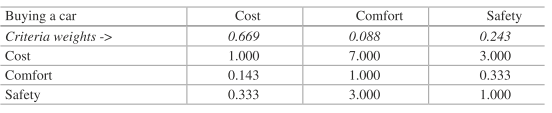
\includegraphics[scale = 1]{img/Kriterien.png}
	\quelle{\cite[S.12]{Mu.2018}}
	\caption{Prioritäten als Faktoren}
	\label{img:crit}
\end{figure}
Danach werden wieder die Summen der Spalten gebildet und durch die jeweiligen Gewichtungen geteilt. Die Ergebnisse werden aufsummiert und durch die Anzahl der Kriterien $n$ geteilt, um den Durchschnitt zu errechnen (Siehe Abbildung \ref{img:lambda}). \\
\begin{figure}[h!]
	\centering
	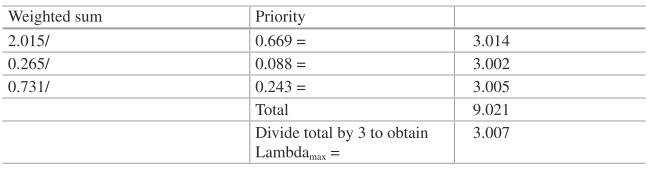
\includegraphics[scale = 0.9]{img/Lambda.png}
	\quelle{\cite[S.14]{Mu.2018}}
	\caption{Berechnung von $\lambda_{max}$}
	\label{img:lambda}
\end{figure} 
Mit $\lambda_{max}$ lässt sich nun der \ac{CIx} von unserer Matrix berechnen. \\
Denn der \ac{CIx} lässt sich wie folgt berechnen:\autocite[Vgl.][S.14]{Mu.2018}
\[CI=\frac{(\lambda_{max}-n)}{(n-1)}\quad \mbox{bzw. für unser Beispiel}\quad CI=\frac{(3.007-3)}{(3-1)}=0.004\]
Damit wir jetzt die \ac{CR} berechnen können, fehlt uns nur noch der \ac{RI}. Hierbei handelt es sich um den \ac{CIx} einer zufällig gefüllten Matrix, welche der Theorie nach sehr inkonsistent sein muss. Saaty stellt praktischerweise schon den durchschnittlichen \ac{CIx} von 500 zufällig gefüllten Matrizen zur Verfügung (Siehe Abbildung \ref{img:ri}).\\
\begin{figure}[h!]
	\centering
	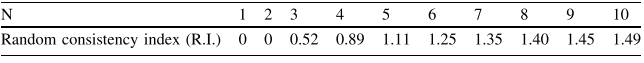
\includegraphics[scale = 0.9]{img/RI.png}
	\quelle{\cite[S.9]{Saaty.2012}}
	\caption{Durchschnittlicher RI}
	\label{img:ri}
\end{figure}\\
Diese sind nach $n$ geordnet und müssen jetzt nur noch in unsere Formel $CR=\frac{\mbox{\ac{CIx}}}{\mbox{\ac{RI}}}$ eingesetzt werden.
\[CR=\frac{\mbox{\ac{CIx}}}{\mbox{\ac{RI}}}=\frac{0.004}{0.52}=0.008\]
Es zeigt sich das $0.008<0.10$. Somit ist die kardinale Konsistenz gegeben, und es kann fortgefahren werden. Sollte dies nicht gegeben sein, muss die Matrix noch einmal überarbeitet werden, um die inkonsistente Stellen zu eliminieren.\autocite[Vgl.][S.108]{Fink.2006}
\subsubsection{Gewichtung der Alternativen}
Nach der Gewichtung der Kriterien werden in diesem Arbeitsschritt die Gewichtungen für die Alternativen berechnet. Die Alternativen werden wie die Kriterien vorher paarweise verglichen, allerdings immer im Hinblick auf ein Kriterium. Hat man also zum Beispiel 3 Kriterien, werden die Alternativen 3 mal im Hinblick auf die Kriterien verglichen. Am Ende entstehen dann 3 Matrizen. 
\begin{figure}[h!]
	\centering
	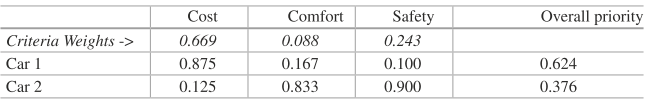
\includegraphics[scale = 0.9]{img/All.png}
	\quelle{\cite[S.19]{Mu.2018}}
	\caption{Modellsynthese}
	\label{img:all}
\end{figure}
Diese werden zusammengefasst und die einzelnen Spalten mit den jeweiligen Prioritäten der Kriterien multipliziert\autocite[Vgl.][S.19]{Mu.2018} (siehe Abbildung \ref{img:all}). Abschließend werden die Summen der Zeilen gebildet. Die Ergebnisse sind dann die globalen Prioritäten und geben die abschließende Reihenfolge der Alternativen an. 
\subsubsection{Sensitivitätsanalyse}
Diese abschließenden Prioritäten sind sehr stark von der Gewichtung der Kriterien beeinflusst.\autocite[Vgl.][S.19]{Mu.2018} Aufgrund dessen wird als letzter Schritt, vor der abschließenden Bewertung, noch eine Sensitivitätsanalyse durchgeführt. Mithilfe dieser wird geprüft, wie \enquote{robust} das Ergebnis der Analyse ist.\autocite[Vgl.][S.20]{Mu.2018} \enquote{Ziel ist es, durch die systematische Verlagerung von Kriteriengewichten Grenzen zu bestimmen, bei denen sich die Reihung von Alternativen umkehrt.}\autocite[S.111]{Fink.2006}\\ 
Getestet wird dies, indem der letzte Schritt der Analyse noch einmal mit veränderten Gewichtungen vorgenommen wird. Was passiert also bei (a) gleichen Gewichtungen, und (b) welche Gewichtung führen zu gleichen Prioritäten?\autocite[Vgl.][S.20]{Mu.2018}\\
Zuerst werden die Gewichtungen aller Kriterien gleichgesetzt. Bei 3 Kategorien würde dies eine jeweilige Gewichtung von $0.333$ bedeuten.\\
Um den \enquote{Break-Even Punkt}\autocite[S.21]{Mu.2018} der Prioritäten zu berechnen kann man sich mithilfe des Ergebnisses aus (a) herantasten. Durch das wiederholte Umstellen der Prioritäten ist es möglich, den \enquote{Break-Even Punkt} zu berechnen. Abschließend werden die Ergebnisse analysiert. \enquote{Führen bereits geringfügige Veränderungen der Kriteriengewichte zu einer [Umkehr der Prioritäten], so ist das ein Hinweis auf ein instabiles Ergebnis. In einem solchen Fall ist es ratsam, den Beurteilungsprozess zu wiederholen bzw. zu überprüfen.}\autocite[S.111]{Fink.2006}
\subsubsection{Finale Entscheidung}
Nachdem alle Schritte vollzogen sind, kann eine finale Entscheidung gefällt werden. Dafür werden die Ergebnisse der Analyse, der Konsistenzanalyse und der Sensitivitätsanalyse einbezogen, um eine aussagekräftige Entscheidung zu treffen, welche Alternative das festgelegte Ziel in Schritt 1 am besten erfüllt.
\section{Versionsverwaltungssysteme}\label{vcs}
In der heutigen Softwareentwicklung besteht ein Projekt aus vielen Quellcode-Dateien, die ständig neu erstellt und verändert werden. Um jegliche Veränderungen an dem Quellcode zu dokumentieren und nachvollziehen zu können, wird ein Versionskontrollsystem (Version Control System; VCS) genutzt.\autocite[Vgl.][S.6]{Baerisch.2005}  
Dieses ermöglicht es dem Entwickler beispielsweise, Weiterentwicklungen durchzuführen, während parallel an der aktuellen Version Fehler behoben werden. Darüber hinaus erlaubt eine Versionsverwaltung dem Entwickler, Änderungen mit anderen zu teilen und Änderungen von verschiedenen Personen zusammenzuführen.\autocite[Vgl.][S.9]{Kleine.2012} \\
Ein VCS bietet die Möglichkeit, Änderungen von Informationen beispielsweise an einem Quellcode zu organisieren und zu verwalten. \autocite[Vgl.][S.1]{Pilato.2009}
Die wachsende Sammlung an Informationen dient als „Repository (Lager), Projektgeschichte, Kommunikationsmedium und Werkzeug zur Team- und Produktverwaltung“.\autocite[][S.1]{Loeliger.2010} In einer Versionsverwaltung lagern somit nicht nur die Quelldateien, sie dient auch als Kernstück für ein ganzes Entwicklungsprojekt. \\
Zentrale Aufgaben der Versionsverwaltung sind der Zugriff auf historische Versionen der Dateien, Aufzeichnung der Änderungen in einem Log und die Entwicklung und Pflege eines Repository mit Inhalten. Die Aufbewahrung von älteren Versionen ist gerade in der Softwareentwicklung wichtig, da Software nach dem „Probierprinzip“\autocite[][S.9]{Versteegen.2003} entwickelt wird. Auf eine neue Entwicklung folgt ein anschließender Test. Es werden so lange Anpassungen durchgeführt und getestet, bis das optimale Ergebnis erreicht wurde.\autocite[Vgl.][S.9]{Versteegen.2003}
Ein Tool zur Sourcecodeverwaltung ermöglicht zudem das Management von Änderungen und den Zugriff von mehreren Entwicklern am gleichen Projekt.\autocite[Vgl.][S.1]{Loeliger.2010} Dies fördert die kollaborative Zusammenarbeit an einem Projekt, da parallel unterschiedliche Entwicklungen von mehreren Personen getätigt werden können. Gerade bei der Arbeit in einem Team muss die Möglichkeit der parallelen Entwicklung gegeben sein, da sich sonst die Entwickler in ihrer Arbeit gegenseitig beeinträchtigen.
\section{Continuous Practices}\label{CP}
Wie bewältigt man die größer werdende Nachfrage von Unternehmen und dem eigenen Management nach kürzerer Time-to-Market (also der Zeit von der Entwicklung bis zum fertigen Produkt) und einer erhöhten Flexibilität und Agilität bei der Entwicklung?\autocite{Capgemini.2017}\\ Continuous Integration, Continuous Delivery und Continuous Deployment (Auch Continuous Practices genannt) sind Techniken, um genau diesen Prozess zu unterstützen.  Sie bieten die Möglichkeit, die Geschwindigkeit des Entwicklungsprozesses zu erhöhen, ohne Qualität einzubüßen.\autocite[Vgl.][S.2]{Shahin.2017}
Die Idee hinter Continuous Integration ist dabei nicht sonderlich neu. Bereits in den 90er Jahren wurde die Idee im größeren Kontext von Extreme Programming und dem Agilen Manifest erwähnt.\autocite[Vgl.][S.2]{Stahl.2018} Auch die grundlegende Idee, eine große Aufgabe in viele kleine Teile zu zerlegen und diese dann einzeln zu bearbeiten, ist nicht neu.\\ Über die Jahre hat sich die Idee weiterentwickelt und wurde von immer mehr Entwicklerteams aufgegriffen. Später kamen dann noch Continuous Delivery und Continuous Deployment hinzu, die mithilfe von Automatisierung den Prozess weiter ausbauten und beschleunigten. Die Abgrenzung zwischen den Begriffen ist dabei nicht genau definiert, weswegen für viele zum Beispiel Teile der Continuous Delivery noch zu Continuous Integration gehören und für andere wiederum nicht. Insgesamt sollen aber alle Continuous Practices zu positiven Veränderungen führen:\autocite[Vgl.][S.2]{Shahin.2017}
\begin{itemize}
	\item Häufigeres und schnelleres Feedback aus dem Entwicklungsprozess und vom Kunden selbst 
	\item Erhöhte Releasezyklen mit stabilen Produkten führt zu erhöhter Produktqualität und verbesserter Kundenzufriedenheit
	\item Manuelle Aufgaben werden automatisiert
\end{itemize}
Im Folgenden wird nun auf die drei Hauptpractices im Detail eingegangen: Continuous Integration, Continuous Delivery und Continuous Deployment. Es existieren noch einige weitere Begriffe, allerdings sind die drei am bekanntesten und sind dementsprechend am häufigsten im Einsatz. Ihre Funktionen werden beschrieben und von dem abgegrenzt was sie nicht sind. 
\subsection{Continuous Integration}
Continuous Integration ist wohl die bekannteste aller Practices und wird immer wieder als Synonym für alle Continuous Practices genannt.\autocite[Vgl.][S.12]{Stahl.2018} Dabei ist es per Definition nur \enquote{eine Softwarenetwicklungspraktik, bei der Entwickler, aus einem Team, ihre Veränderungen häufig in das Projekt integrieren. Mindestens einmal täglich}\autocite[S.12]{Stahl.2018}\\
Dies ist wichtig wenn die Größe des Entwicklungsteams über 1 wächst. Denn sobald mehrere Leute an einem Projekt arbeiten, wird es schwieriger, die Veränderungen des einen Entwicklers mit denen des anderen zu verknüpfen und das Programm zum Laufen zu kriegen.\autocite[Vgl.][S.4]{Stahl.2018}\\ Mann kann es vergleichen mit dem gemeinsamen Schreiben vieler Autoren an einem sehr langen Roman. Die Geschichte und alle Charaktere müssen konsequent geschrieben sein, damit das Buch verständlich ist. Je mehr Autoren mitarbeiten, umso schwieriger wird es, die einzelnen Teile zusammenzuführen.\\ Das gleiche Problem tritt auch in der Softwareentwicklung auf und wird komplizierter mit jedem Entwickler, der dazu kommt. Außerdem wird es umso schwieriger, wenn Veränderungen von einem Entwickler länger zurückgehalten werden. Je umfangreicher die Veränderungen sind, die eingebracht werden, umso schwieriger wird es, diese zu integrieren.\\ Dies bringt uns wieder zur Definition vom Anfang. Es geht nicht darum, so oft und schnell wie möglich zu integrieren, sondern um die Häufigkeit und Regelmäßigkeit.\autocite[Vgl.][S.3]{Stahl.2018} Darüber hinaus werden die Veränderungen automatisch getestet, um eine sichere Basis zu haben, auf der alle arbeiten können.\\ Continuous Integration führte zu einem Paradigmenwechsel. Ohne Continuous Integration ist die Applikation nicht lauffähig, bis das Gegenteil in Form von Tests oder dem Deployment bewiesen ist. Mit Continuous Integration funktioniert die Applikation erwiesenermaßen (Automatische Builds, Tests etc.). Und es wird sofort bemerkt, wenn etwas nicht mehr funktioniert.\autocite[Vgl.][S.40]{Farley.2010}\\ Es beschleunigt den gesamten Entwicklungsprozess, da weniger Ressourcen für das Integrieren gebraucht werden. Des Weiteren bildet Continuous Integration die Grundlage für Continuous Delivery und Continuous Deployment. Ohne kontinuierliches Integrieren bringen diese beiden Practices keinen Vorteil.
\subsection{Continuous Delivery}
2010 haben Jez Humble und David Farley\autocite{Farley.2010} die Idee der Continuous Integration weiterentwickelt. Sie gehen von der Basis, welche durch die Veränderungen der Entwickler regelmäßig gepflegt wird, aus, und behandeln jede Bearbeitung dieser Basis als möglichen Releasekandidaten.\autocite[Vgl.][S.5]{Stahl.2018} Mithilfe einer automatisierten Pipeline, also einer Abfolge von Programmausführungen auf die Codebasis, wird aus dem Code ein lauffähiges Programm. Das Ziel dieses Prozesses ist es, immer einen lauffähigen und getesteten Releasekandidaten zu haben, welcher bei Bedarf, zum Beispiel um dem Kunden den Fortschritt zu zeigen, manuell deployed oder auch released werden kann.\autocite[Vgl.][S.16]{Stahl.2018}
\begin{figure}[h!]
	\centering
	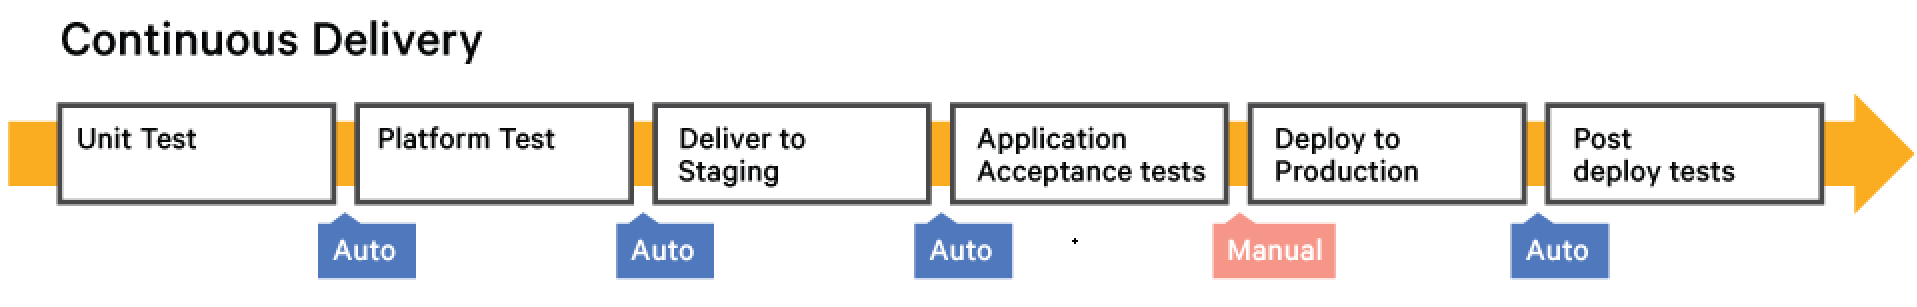
\includegraphics[scale = 0.3]{img/CDE.png}
	\quelle{\cite{Puppet.2013}}
	\caption{Continuous Delivery Pipeline}
	\label{img:cde}
\end{figure}\\
In Abbildung \ref{img:cde} findet sich eine auf das wesentliche herunter gebrochenen Beispielpipeline. Dabei fehlt der wichtige erste Schritt aus Continuous Integration: das tatsächliche Integrieren.\\ Hier stoßen wir bereits auf die erste Technologie. Damit das Integrieren von vielen Veränderungen von verschiedenen Entwicklern gleichermaßen geordnet und protokolliert abläuft, wird heutzutage eigentlich immer ein Versionsverwaltungssystem (\ref{vcs}) genutzt.\autocite[Vgl.][S.2]{Arachchi.2018} Dort wird der gesamte Code zentral verwaltet und bildet damit die beschriebene Basis für alles weitere. Des Weiteren dient es auch als Auslöser zum Start der gesamten Pipeline. Veränderungen werden automatisch vom System erkannt, welches dann die automatische Pipeline anstößt. Bei dem System handelt es sich meistens um einen dedizierten CI/CD Server, welcher die Pipeline dann entsprechend ihres Aufbaus abarbeitet.\autocite[Vgl.][S.2]{Meyer.2014}\\ Noch vor dem ersten Schritt aus Abbildung \ref{img:cde} wird die Applikation erst einmal gebaut. Das heißt, etwaige Abhängigkeiten werden installiert, und der Quellcode wird in einen ausführbaren Programmcode übersetzt.\autocite[Vgl.][S.36]{Farley.2010} Des Weiteren wird mit diesem Schritt auch der erste Test der Applikation durchgeführt. Wenn die Syntax des Quellcodes nicht stimmt, würden hier die ersten Fehler auftreten.\autocite[Vgl.][S.37]{Farley.2010}\\ Theoretisch fallen diese Schritte noch in den Bereich von Continuous Integration. Sie werden erst hier beschrieben, damit ein Gesamtbild über den Ablauf gegeben werden kann.\\
Nachdem die Applikation gebaut ist, kann sie getestet werden. Hierfür können verschiedene automatisierte Testverfahren eingesetzt werden.
\begin{itemize}
	\item \texttt{Unit-Tests(Komponententests)} \\Unit-Tests überprüfen, ob die von den Entwicklern geschriebenen Komponenten so arbeiten, wie diese es beabsichtigen. Zum Beispiel ob ein Input den gewünschten Output liefert.\autocite[Vgl.][S.21]{Westphal.2012} Zur Qualitätssicherung wird eine sehr häufige Ausführung der Komponententests angestrebt. Dabei ist es üblich, dass der Test in der gleichen Sprache wie das Testobjekt geschrieben wird.
	\item  \texttt{Statische Codeanalyse}\\ \enquote{Die statischen [Code]Analyseverfahren [dienen der] Syntax-, Konsistenz- und Vollständigkeitsprüfung.}\autocite[S.264]{Bommer.2008} Statische Tests sorgen dafür, dass Fehler und potenzielle Fehlerquellen frühzeitig erkannt werden. Dabei steht die Prävention von Fehlern im Vordergrund. Sie sollen so früh wie möglich erkannt werden, um spätere und arbeitsintensive Nachbesserungen zu vermeiden.\autocite[Vgl.][S.263]{Bommer.2008}
	\item  \texttt{End-to-End Tests} \\End-to-End Tests werden genutzt, um Abläufe innerhalb einer Applikation vom Anfang bis zum Ende zu testen. Der Zweck von End-to-End Tests ist dabei die Simulation von echten Nutzerszenarien und die Validierung des Systems und der Datenintegrität.\autocite[Vgl.][S.250]{Bommer.2008} Dabei werden Szenarien aus der echten Welt getestet, wie zum Beispiel die Kommunikation über die API, die Kommunikation mit der Datenbank und vieles mehr. End-to-End Tests sind dabei sehr arbeitsintensiv, weil bei Änderungen zum Beispiel an der Weboberfläche auch alle End-to-End Tests überarbeitet werden müssen. Diese würden sonst fehlschlagen.\autocite[Vgl.][S.252]{Bommer.2008}
\end{itemize}
 Sollten ein oder mehrere Tests fehlschlagen, wird dies auf dem CI/CD System angezeigt, und der Entwickler kann entsprechende Fehler leicht erkennen und ausbessern. Des Weiteren werden alle eventuell schon installierten Teile auf die Ausgangsbasis zurück gerollt um etwaige Beeinträchtigungen zu vermeiden. Wenn die Veränderung also auf das Entwicklungssystem ausgerollt wird während des Durchlaufs der Pipeline, dann werden alle gemachten Veränderungen verworfen, und das System kann ganz normal weiter funktionieren.\autocite[Vgl.][S.41]{Farley.2010} Wenn alle Tests positiv verlaufen sind, wird die Pipeline fortgeführt.\\
 Der nächste Schritt wäre die Implementierung der getesteten Applikation auf einer sogenannten Staging Umgebung. Dort sind dieselben Voraussetzungen gegeben wie auf der späteren Produktivumgebung.\autocite[Vgl.][S.283]{Farley.2010} Dort kann der Kunde sich die gemachten Veränderungen anschauen und überprüfen. Die Abnahme, also die Bestätigung, dass die Veränderung mit den Interessen des Kunden übereinstimmen, (auch Acceptance Tests genannt) kann entweder manuell oder automatisiert geschehen. Bei manueller Abnahme ist der Arbeitsaufwand ungemein höher, weil bei jeder integrierten Veränderung eine Abnahme gemacht werden muss. Mit automatisierten Acceptance Tests wird der gesamte Prozess beschleunigt und Kosten gespart.\autocite[Vgl.][S.310]{Farley.2010} Acceptance Tests werden ähnlich wie End-to-End Test aufgebaut, um die Usererfahrung abzubilden. Dabei werden die Tests meistens direkt auf dem User Interface ausgeführt. Am Erstellen dieser Tests sind meistens alle Stackeholder der Applikation beteiligt, vom Entwickler bis zum Kunden.\autocite[Vgl.][S.312]{Farley.2010}\\ \\ \\Dabei sind die Testfälle immer gleich aufgebaut\autocite[Vgl.][S.312]{Farley.2010}:
 \begin{itemize}
 	\item\textbf{GIVEN} some initial context,
 	\item\textbf{WHEN} an event occurs,
 	\item\textbf{THEN} there are some outcomes.
 \end{itemize}
Es wird der Input, die aufgerufene Aktion und das gewünschte Ergebnis beschrieben. Mit dieser Syntax lassen sich alle Testfälle beschreiben.\autocite[Vgl.][S.312]{Farley.2010}\\
Sobald die Acceptance Tests erfolgreich durchgeführt sind, endet die automatische Pipeline. Am Ende steht eine releasefähige Version der Applikation, welche ausreichend getestet und abgenommen wurde. Da die Pipeline bei jeder Veränderung ausgelöst wird, hat man also immer ein aktuelle lauffähige Version, die jederzeit präsentiert oder auch released werden kann. Dem Rollout auf das Produktivsystem steht jetzt hoffentlich nur noch ein Knopfdruck im Weg, wenn der Deploymentprozess entsprechend automatisiert ist. Wenn der Kunde oder das Management dann die Freigabe zum Release erteilt, geht alles ganz schnell.\autocite[Vgl.][S.289]{Farley.2010}
\subsection{Continuous Deployment}
Continuous Deployment geht noch einen Schritt weiter und sagt:\enquote{Jede Veränderung soll direkt auf das Produktivsystem deployed werden}\autocite[Vgl.][S.17]{Stahl.2018} Damit automatisiert Continuous Deployment den letzten Schritt, den Continuous Delivery als manuelle Tätigkeit übriglässt (siehe Abbildung \ref{img:cde2}).
\begin{figure}[h!]
	\centering
	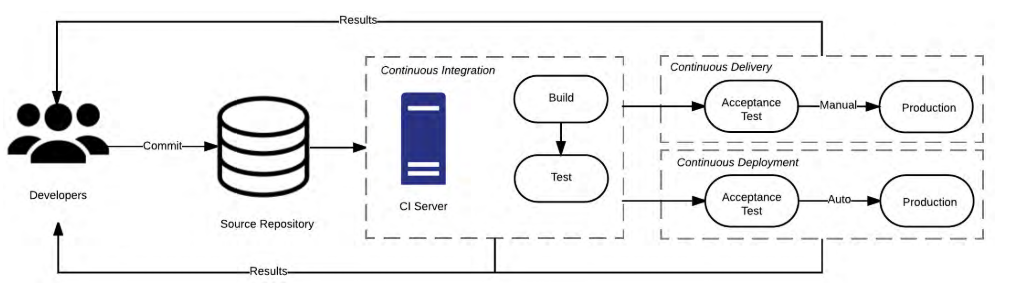
\includegraphics[scale = 0.6]{img/CDE2.png}
	\quelle{\cite[S.3]{Shahin.2017}}
	\caption{Vergleich Continuous Delivery \& Continuous Deployment}
	\label{img:cde2}
\end{figure}\\
 Wo Continuous Delivery immer einen Releasekandidaten in der Hand hat , welcher jederzeit released werden kann, geht Continuous Deployment diesen Schritt weiter und tut es.\autocite[Vgl.][S.17]{Stahl.2018} Bevor man allerdings diesen Schritt geht, ist einiges zu beachten. Es sollte darauf geachtet werden, dass es während des Deploymentprozesses zu keinen Downtimes kommt und der Wechsel für den Nutzer praktisch nicht bemerkbar ist. Hierfür kann sich des Blue-Green Deploymentansatzes bedient werden.\autocite[Vgl.][S.407]{Farley.2010}
\begin{figure}[h!]
 	\centering
 	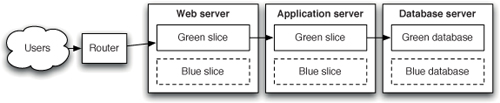
\includegraphics[scale = 1]{img/blue.jpg}
 	\quelle{\cite[S.407]{Farley.2010}}
 	\caption{Blue-Green Deployment}
 	\label{img:blue}
\end{figure}
Bei diesem Ansatz werden zwei Versionen der gleichen Applikation nebeneinander betrieben. Die grüne Applikation (Siehe Abbildung \ref{img:blue}) stellt in diesem Beispiel die alte Version dar, welche zurzeit noch in Betrieb ist. Die blaue Applikation wird währenddessen parallel zur grünen hochgefahren und startbereit gemacht. Sobald die blaue einsatzbereit ist, wird der Traffic von der grünen Applikation auf die blaue gelenkt. Am einfachsten funktioniert dies, wenn dem Ganzen ein Router vorgeschaltet ist, welcher den Traffic lenken kann (siehe Abbildung \ref{img:blue}).\autocite[Vgl.][S.407]{Farley.2010} Der Nutzer bekommt von dem Wechsel kaum etwas mit, und die Applikation muss keine Downtime in Kauf nehmen. Außerdem kann im Fall eines Fehlers in der blauen Applikation sofort wieder auf die grüne gewechselt werden. Einzig bei dem Wechsel der Datenbanken kann es zu Komplikationen kommen, da die Daten aus der grünen Applikation auf die Datenbank der blauen kopiert werden müssen.\autocite[Vgl.][S.407]{Farley.2010}\\  
Für den gesamten Prozess des Continuous Deployments ist allerdings zu beachten, dass das Deployment nicht immer so einfach funktioniert. Ein großer Teil der heutzutage eingesetzten Software wird noch vom User selbst installiert, und Veränderungen können nicht so einfach für alle released werden. Mit dem wachsenden Anteil von \enquote{X as a Service}-Angeboten\autocite[S.18]{Stahl.2018} sollte sich dies allerdings bald ändern\autocite[Vgl.][S.18]{Stahl.2018} Allgemein gesagt ist Continuous Deployment also die weitergeführt Idee von Continuous Delivery und hilft dabei, den Prozess weiter zu beschleunigen.
\subsection{DevOps}\label{devops}
Der Begriff DevOps kommt in den letzten Jahren immer häufiger auf\autocite{Sauce.2018} und wird dabei auch oft im Zusammenhang mit Continuous Integration, Continuous Delivery und Continuous Deployment genannt. DevOps entstand als Reaktion auf die größer werdende Lücke zwischen der Entwicklung einer Software und dem tatsächlichen Betrieb dieser.\autocite[Vgl.][S.22]{Stahl.2018}\\ Dieser Bewegung schlossen sich immer mehr Leute an, die ihre Erfahrungen mit dem Integrieren von der Entwicklung in die Operations dort einbrachten. Über die Zeit entwickelte sich DevOps weiter, und je bekannter es wurde, umso öfter wurde es mit Continuous Integration, Continuous Delivery und Continuous Deployment genannt und miteinander vertauscht.\autocite[Vgl.][S.23]{Stahl.2018} Im Kern ist DevOps eine Sammlung aus \enquote{Prinzipien, Werten, Methoden und Praktiken}\autocite[S.23]{Stahl.2018}. Zu diesen Praktiken zählen auch Continuous Integration, Continuous Delivery und Continuous Deployment. 
\begin{figure}[h!]
	\centering
	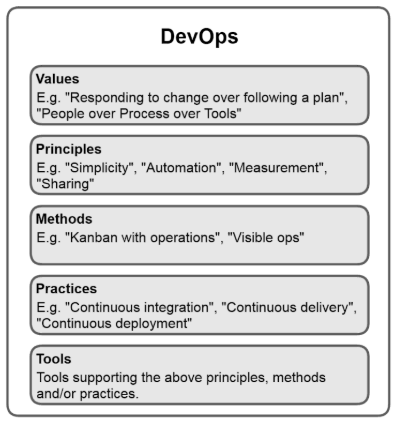
\includegraphics[scale = 0.7]{img/DEVOPS.png}
	\quelle{\cite[S.24]{Stahl.2018}}
	\caption{Zusammensetzung DevOps}
	\label{img:devops}
\end{figure}Diese sowieso die anderen Inhalte (siehe Abbildung \ref{img:devops}) von DevOps helfen dabei, die Entwicklung und die Operations miteinander zu verknüpfen und so die allgemeine Zufriedenheit und Produktivität zu verbessern. Dafür muss die sogennante \enquote{DevOps-Kultur} allerdings erst einmal in allen Ecken eines Unternehmens ankommen.\autocite[Vgl.][S.23]{Stahl.2018} Denn die Implementation von DevOps ist nicht immer einfach. Viele Unternehmen treffen dabei auf Probleme (siehe \cite{Claranet.2016}). Fast 50\% der Unternehmen gaben an, dass die Implementierung an einigen Punkten stockte, aufgrund von mangelnden Qualifikation der Mitarbeiter, fehlender Zeit, und weil es zu Konflikten mit alten Prozessen innerhalb des Unternehmens kam.\autocite[Vgl.][]{Claranet.2016} Wenn DevOps allerdings richtig betrieben wird, ermöglicht es eine Hebelwirkung, die dem gesamten Unternehmen hilft.\autocite[Vgl.][S.24]{Stahl.2018} 
\chapter{Praktische Umsetzung}
In diesem Teil der Arbeit liegt der Fokus auf der praktischen Anwendung. Es wird das Analyseverfahren ausgewählt und dann auf die Problemstellung angewendet. Doch zuerst folgt eine kurze Einführung in das Projektumfeld.
\section{Projektumfeld}
Diese Bachelorarbeit findet im Umfeld der Atos Information Technology GmbH statt. Das Unternehmen ist die deutsche Tochtergesellschaft des französischen IT-Dienstleisters Atos SE. Die Atos SE ist ein internationaler IT-Dienstleister mit Hauptsitz in Paris. Das Unternehmen deckt unter anderem die Geschäftsfelder Beratungs- und Technologieservices, Systemintegration und Outsourcing-Dienstleistungen ab.\\
Die Abteilung AITs-B\&PS-GER-TEC-AM CAP DB APP NordWest, in welcher die Arbeit geschrieben wird, betreibt dabei größtenteils klassische Service Delivery, also die Umsetzung und Lieferung von Kundenanfragen. Mittlerweile gibt es aber auch ein kleines Team von Entwicklern, dass sich agil nach DevOps (siehe \ref{devops}) organisiert und proaktiv neue kleinere Projekte angeht. Dabei fokussieren die Entwickler sich besonders auf neue Technologien, wie zum Beispiel Angular, NodeJS und auch \ac{CI}/\ac{CDE}/\ac{CD}.\\ 
Dabei haben sie gemerkt, dass Continuous Practices einen großen Mehrwert für sie bringen. Jederzeit eine getestete und lauffähige Version ihrer Applikation in der Hand zu haben, hilft ihnen sehr, da sie in Sprints arbeiten. Das heißt, sie haben vorher abgestimmte Arbeitspakete, welche sie dann in einem bestimmten Zeitraum (meistens eine Woche) abarbeiten, um am Ende eine Review mit dem Kunden durchzuführen. Mithilfe der Continuous Practices gibt es immer eine lauffähige Version der Applikation, welche dem Kunden präsentiert werden kann. Außerdem können sie sich vollkommen auf die Entwicklung konzentrieren, da alles andere automatisch im Hintergrund abläuft.\\ 
Diese Vorteile möchte die Abteilung nun auch anderen zur Verfügung stellen. Mit \ac{CI}/\ac{CDE}/\ac{CD} as a Service möchten sie internen so wie externen Kunden die Möglichkeit bieten, einfach in Continuous Practices einzusteigen und damit ihre Entwicklung zu verbessern. Des Weiteren eröffnet sich dadurch eine neue Einnahmequelle für die Abteilung.
%\section{Zieldefinition}
\section{Auswahl der vergleichenden Analysemethode}
Damit der Service erstellt werden kann muss sich zuerst für ein \ac{CI}/\ac{CDE}/\ac{CD}-Tool entschieden werden. Doch wie entscheidet man sich für eine Alternative? Mit der Auswahl von Alternativen beschäftigt sich der Forschungsbereich der Entscheidungstheorie. Dort bieten sich verschiedene Methoden an um Entscheidungen zu treffen. Dabei teilt sich die Entscheidungstheorie in zwei Teilgebiete auf\autocite[Vgl.][S.1]{Laux.2014}:
\begin{itemize}
	\item Die präskriptive (normative) Entscheidungstheorie
	\item Die deskriptive Entscheidungstheorie 
\end{itemize}
Die deskriptive Entscheidungstheorie beschäftigt sich dabei nur damit wie und warum Entscheidungen in der Realität getroffen werden. \enquote{Ihr Ziel ist es, empirisch gehaltvolle Hypothesen über das Verhalten von Individuen und Gruppen im Entscheidungsprozess zu finden, mit deren Hilfe bei Kenntnis der jeweiligen konkreten Entscheidungssituation Entscheidungen prognostiziert bzw. gesteuert werden können.}\autocite[S.4]{Laux.2014}\\
Aus diesem Grund wird sich diese Arbeit im Bereich der präskriptiven Entscheidungstheorie bewegen. Es soll nicht herausgefunden werden wie Entscheidungen gefällt werden sondern es wird nach einem Modell gesucht, dass dabei hilft rational eine Entscheidung zu treffen. Dafür kommt nur die präskriptive Entscheidungstheorie infrage. Denn \enquote{sie will Ratschläge für die Lösung von Entscheidungsproblemen erteilen, also Antwort geben auf die Frage, was ein Entscheider in unterschiedlichen Entscheidungssituationen tun soll.}\autocite[S.4]{Laux.2014} \\
Auch der Bereich der \enquote{\ac{MCDA}} gehört zur präsriptiven Entscheidungstheorie. \ac{MCDA} befasst sich, wie der Name schon aussagt, mit unterschiedlichen Verfahren die sich dadurch auszeichnen, dass sie kein einzelnes übergeordnetes Kriterium, sondern mehrere unterschiedliche Kriterien nutzen, um Alternativen für die Entscheidungsfindung zu evaluieren. Da in die Entscheidung für ein \ac{CI}/\ac{CDE}/\ac{CD}-Tool viele Kriterien mit einfließen sind die Verfahren der \ac{MCDA} bestens geeignet um eine Entscheidung zu treffen und die Alternativen zu evaluieren.\\ \\ Zu den bekanntesten Verfahren gehören:
\begin{itemize}
	\item Nutzwertanalyse
	\item AHP-Analyse (Analytic Hierarchy Process)
	\item TOPSIS (Technique for Order Preference by Similarity to Ideal Solution)
\end{itemize}
Diese drei kommen dabei in die nähere Auswahl für die Anwendung in der späteren Analyse. Alle haben ihre Vor- und Nachteile, die im Folgenden evaluiert werden.
\subsection{Nutzwertanalyse}
Die Nutzwertanalyse ist eine bekannte Methode (besonders in Deutschland) um Alternativen anhand einer Fragestellung zu vergleichen. Dafür wird das Grundproblem/Fragestellung fragmentiert und in Kriterien umgewandelt. 
\begin{figure}[h!]
	\centering
	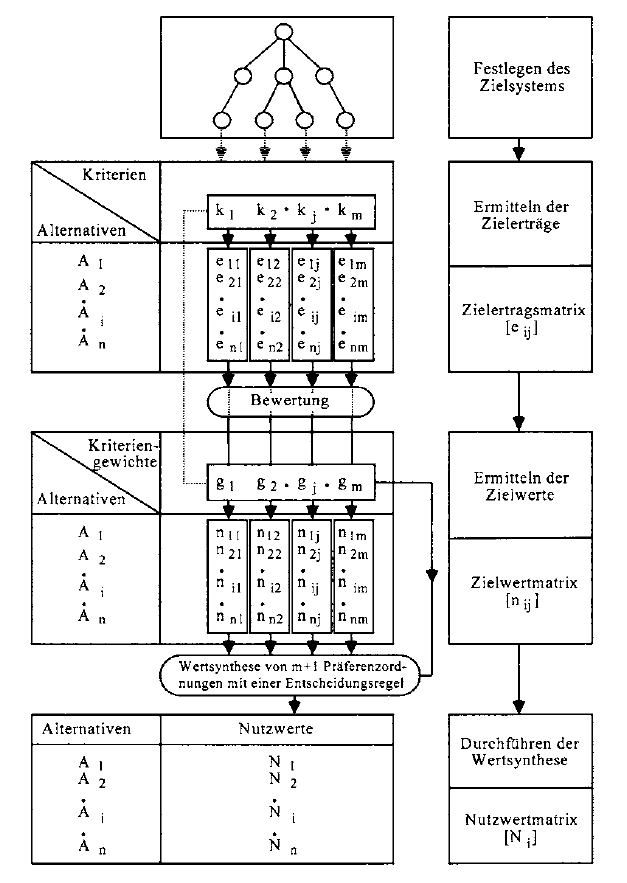
\includegraphics[scale = 0.7]{img/NUTZ.png}
	\quelle{\cite[S.112]{Fink.2006}}
	\caption{Vorgehensweise bei der Nutzwertanalyse}
	\label{img:nutz}
\end{figure}
Diese Kriterien werden gewichtet und die Alternativen werden im Hinblick auf jedes einzelne Kriterium bewertet. Am Ende steht eine Gesamtbewertung für jede Alternative, anhand die Reihenfolge dieser bestimmt wird.\\
Dabei ist die Nutzwertanalyse sehr einfach anzuwenden. Es wird keine große Rechenleistung benötigt um die Werte auszurechnen. Des Weiteren ist sie einfach erweiterbar, wenn man also eine Alternative oder ein Kriterium nachträglich hinzufügen will kann dies ohne große Auswirkungen geschehen.\\
Allerdings führt die Einfachheit auch zu Schwachpunkten. Zum Beispiel kann durch die Gewichtung der Kriterien schnell Subjektivität in den Prozess hineinkommen, da sie meistens den größten Einfluss auf das Ergebnis haben. Außerdem ist es nicht möglich eine Konsistenzprüfung der Daten durchzuführen um auf etwaige Inkonsistenzen zu prüfen. Somit ist die Nutzwertanalyse eine einfache und schnelle Möglichkeit um Alternativen zu vergleichen, welche allerdings auch ihre Schwächen hat. 
\subsection{AHP-Analyse}
Die AHP-Analyse (Analytic Hierarchy Process) von Thomas L. Saaty aus den 1970er Jahren ist sehr ähnlich zu der Nutzwertanalyse aufgebaut. Der große Unterschied liegt in der Gewichtung und Bewertung der Alternativen. Diese entstehen nicht wie in der Nutzwertanalyse durch einfaches Setzten der Werte sondern durch paarweise Vergleiche. Jedes Kriterium wird einzeln mit jedem anderen anhand einer Skala verglichen um eine objektive Gewichtung der Kriterien zu erreichen. Das selbe passiert mit den Alternativen. Jede Alternative wird im Vergleich zu den anderen Kriterien und im Hinblick auf jedes einzelne Kriterium bewertet. Dabei können verschiedene Skalen zum Einsatz kommen, allerdings empfiehlt Saaty selber die Skala von 1 bis 9 mit wörtlich formulierten Abstufungen (siehe Abbildung \ref{img:scale}) Eine genaue Beschreibung des Ablaufs einer AHP-Analyse findet sich in Kapitel \ref{ahp}. Dort wird der gesamte Ablauf einer AHP-Analyse beschrieben. \\Der Vorteil dieser Methode liegt dabei in ihrer Objektivität. Durch die Paarvergleiche wird versucht die Subjektivität möglichst außen vor zu lassen. Der Entscheider wird durch die Paarvergleiche gezwungen sich das Problem in allen Details anzuschauen. Des Weiteren führt die AHP-Analyse eine Konsistenzprüfung durch um mögliche Fehler in der Logik zu finde. Wenn zum Beispiel $A > B$ gilt und $B > C$ dann muss auch $A > C$ gelten.\\
Durch die Paarvergleiche und Matrizenrechnung ist die AHP-Analyse allerdings auch recht aufwändig. Sowohl zeitlich als auch mathematisch. Außerdem ist es schwierig und aufwändig im Nachhinein noch weitere Alternativen oder Kriterien hinzuzufügen.
Zusammengefasst ist die AHP-Analyse eine gut Möglichkeit um objektiv und detailliert Entscheidungen zu treffen.
\\
\subsection{TOPSIS}
Die TOPSIS (Technique for Order Preference by Similarity to Ideal Solution) Methode hat eine andere Herangehensweise als die Nutzwertanalyse und die AHP-Analyse. Sie definiert während des Prozesses eine obere und untere Grenze. Damit ist sowohl die schlechteste als auch die beste mögliche Bewertung einer Alternative gemeint. Diese Grenzen werden aus einer Matrix gewonnen die während des Prozesses erstellt wird (siehe Abbildung \ref{img:topsis}). Sie ergibt sich dabei aus der Bewertung der Alternativen im Hinblick auf die Kriterien.
\begin{figure}[h!]
	\centering
	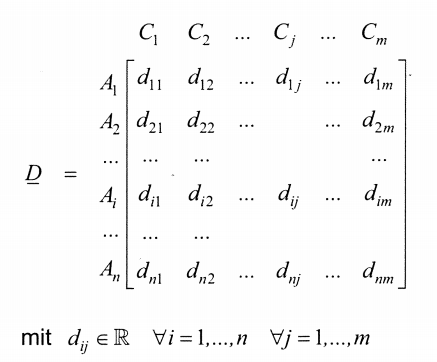
\includegraphics[scale = 0.7]{img/TOPSIS.png}
	\quelle{\cite{Peters.2007}}
	\caption{Matrix mit Alternativen und Kriterien}
	\label{img:topsis}
\end{figure}\\
In den Spalten finden sich jeweils die Bewertungen aller Alternativen in Bezug auf ein Kriterium. Logischerweise stehen dann in den Zeilen die Bewertung einer Alternative im Bezug auf alle Kriterien. Für jede Spalte wird dann das Minimum und Maximum gesucht um dadurch sowohl die obere als auch die untere Grenze zu bestimmen. Dabei ist zu beachten, dass die obere Grenze von Kriterium zu Kriterium unterschiedlich sein kann, da bei manchen Kriterien eine niedrige Bewertung als positiv angesehen wird. Als Letzter Schritt werden die euklidischen Distanzen zwischen den Bewertungen der Alternativen und denen der oberen und unteren Grenzen bestimmt. Die Alternative mit der geringsten Gesamtdistanz zur oberen Grenze oder der größten Gesamtdistanz zur unteren ist damit dann die beste Alternative. Außerdem ergibt sich dadurch eine Reihenfolge der Alternativen.\\
Die TOPSIS Methode ist eine gute Möglichkeit um schnell eine Reihenfolge aus den vorhandenen Bewertungen zu erhalten. Außerdem benötigt sie wie die Nutzwertanalyse keine zusätzlichen Hilfsmittel und ist mathematisch einfach zu berechnen. Allerdings nutzt sie für die Bewertung der Alternativen eine Methode ähnlich zur Nutzwertanalyse, wodurch auch die Vor- und Nachteile dieser mit einfließen.
\section{Kriterienkatalog}
\section{Vorstellung der Alternativen}
\section{Analyse}
\subsection{Aufstellung des Zielsystems}
\subsection{Gewichtung der Kriterien}
\subsection{Gewichtung der Alternativen}
\subsection{Berechnung der Gesamtgewichtung}
\subsection{Bewertung der Alternativen}
\section{Handlungsempfehlung}
\chapter{Zusammenfassung}
\section{Fazit} 
\section{Kritische Reflexion}
